\documentclass{optica-article}

%% Select the journal you're submitting to
%% oe, boe, ome, optcon, opticajournal
\journal{optcon}
% Key:
% Express journals must have the correct journal selected:
% {oe} Optics Express
% {boe} Biomedical Optics Express
% {ome} Optical Material Express
% {optcon} Optics Continuum
% Other Optica journals may use:
% {opticajournal} Applied Optics, Advances in Optics and Photonics, Journal of the Optical Society of America A/B, Optics Letters, Optica, Photonics Research

% Uncomment if submitting to Photonics Research.
% ONLY APPLICABLE FOR \journal{opticajournal}
% \setprjcopyright

% Set the article type
\articletype{Research Article}
% Note that article type is not required for Express journals (OE, BOE, OME and OPTCON)

\usepackage{lineno}
\usepackage{outlines} % Creates nice lists
\usepackage{siunitx} % intuitive way to layout units
\usepackage{nicefrac}
\linenumbers

\begin{document}

\title{Investigation of Retinal Biochemistry with Phasor S-FLIM}

\author{Daniel Martin Geddes,\authormark{1} Rui Wang,\authormark{1,2} and Andrew R. Harvey\authormark{1,*}}

\address{\authormark{1}School of Physics and Astronomy, University of Glasgow, Glasgow, G12 8QQ\\
\authormark{2}Publications Department, Optica Publishing Group, 2010 Massachusetts Avenue NW, Washington, DC 20036, USA\\}

\email{\authormark{*}andy.harvey@glasgow.ac.uk} %% email address is required; see note below about the corresponding author designation

% \homepage{http:...} %% author's URL, if desired

%%%%%%%%%%%%%%%%%%% abstract %%%%%%%%%%%%%%%%
%% [use \begin{abstract*}...\end{abstract*} if exempt from copyright]

\begin{abstract}
Insert Abstract
\end{abstract}
\section{Narrative for Paper}
\begin{itemize}
    \item Quantifying concentration of fluorescent retinal biomarkers can be used to improve the detection of retinal disease and assessing retinal metabolic health
    \item For example: the detection of lipofuscin (A2E) informs the diagnosis of mucular degeneration, Stargaart's disease etc.: mapping FAD offers a new route to mapping oxygen consumption in the eye
    \ fluoresecent signatures of spectra of A2E and FAD occur overlap significantly and also overlap with AGE fluoresence in the eye (which also increases with age). The non-orthogonal spectra and similar fluorescence lifetimes exhibited by these fluorophores coupled with the feint, high noise, fluorescence signal restrict the accuracy, and precision, in this unmixing process.
    \item The fluoresence lifetimes of these flurophores also differ providing an additional scope, when combined with spectral signatures  of FAD, AGE, and A2E to provide enhanced discrimination. This is S-FLIM
    \item S-FLIM has previously been used in labelled samples in microscopy where it has demonstrated \textcolor{red}{explain what the claimed advantage is}. Labelling enables spectra to be selected with low overlap - \textcolor{red}{so one might expect the benefit of FLIM would be less important?}. Phasor S-FLIM involves representation of the spectral lifetime as a phasor - that is the phase of first harmonic of the FFT. Although this works, one would not expect it to be optimal since the correlation of a Cos and Sin with the exponential fit is low - can we quantify it?
    \item For in vivo imaging in the human eye only autofluorescence imaging is possible and the spectral 
   
    \item Spectral unmixing, and SFLIM unmixing methods are compared for their performance in unmixing linear combinations of retinal fluorophores to establish:
    \begin{itemize}
        \item How does noise affect the accuracy of popular unmixing methods : VCA, NMF (Spectral); phasor analysis, fitting (FLIM); and S-FLIM. [Condition Number, error in abundance vs photon counts]
        \item Which method is best suited for unmixing retinal fluorophores and what are the error bounds on the recovery of relative abundances
        \item How can the measurement of the spectra/FLIM/S-FLIM data be optimised - more narrow bands, fewer broad bands, and if so how many, which wavelengths
        \item Do fluorescence lifetimes enhance the unmixing process or are the limited detected photons better 'spent' solely  on FLIM, Spectral Imaging, or SFLIM?
    \end{itemize}
    \item These questions will be addressed by first using a series of simulated and experimental data comprising of linear combinations of spectras with variable abundances and known lifetime:
    \begin{itemize}
        \item Easy - non overlapping Gaussian spectra, with know lifetimes, variable noise levels (establishes that we can implement these techniques and they can work)
        \item Hard - using retinal fluorophores, variable noise, irfs etc
        \item Harder - In Vitro data comprising of 2+ different fluorophores, and a mixture of multiple fluorophores, in capillary tubes
        \item Hardest - In-Vivo data where we unmix the fluorophores in a rat.
    \end{itemize}
\end{itemize}

\section{Introduction}
Current practices in the diagnosis of retinal disease rely on the detection of physical damage to the retinal surface[\textcolor{red}{citation needed}], or structural changes in the retina [\textcolor{red}{citation needed}] through routine clinical imaging or the reports of abnormalities in patient vision. However, at this stage of disease progression any loss of central vision is usually unrecoverable - this motivates the need for imaging techniques capable of assessing retinal health on the metabolic level allowing intervention at the early stages of biochemical dysfunction and improving patient outcomes. 
\\
Measurements of oxygenation in retinal blood vessels using spectral imaging have been reported but the large uncertainty in these measurements is comparable to the variation expected with retinal disease. This reduced sensitivity coupled with the lack of knowledge of oxygen consumption in the surrounding retinal tissue limits clinical applications [\textcolor{red}{citation needed}]. 
\\
Spectral fluorescence imaging offers a more direct assessment of retinal biochemistry by measuring the concentration of fluorescence flavoproteins, such as FAD and NADH, Advanced Glycation End products (AGE), and fluorescent exudates but this is not without its significant challenges. Safe exposure thresholds of phototoxic damage from short wavelengths required for excitation results in images requiring lengthy acquisition times and exhibiting low SNR. This already feint fluorescence signal is often contaminated by fluorescent clutter and scattering from blood vessels meaning that discriminating retinal fluorophores is infeasible using spectral imaging alone.
Instead the fluoresence lifetime - the average time a fluorophore remains in an excited state - is invariant to intensity and can be used to infer pH, FAD and NADH redox reactions, and infer conditions of the local environment. The field of Fluorescence Lifetime Imaging Ophthalmoscopy (FLIO) investigates the benefits of fluorescence lifetime imaging with the diagnosis of retinal disease. In clinical studies, the progression of common retinal diseases such as Age-related Macular Degeneration, Diabetic Retinopathy, and Stargardt's disease were shown to be connected to qualitative changes in the distributions of fluorescence lifetimes across the retina~\cite{schweitzer2007towards, dysli2017fluorescence}. However, quantitative assessments of fluorophore concentrations is yet to be reported.
\\


Spectrally resolved Fluorescence Lifetime Imaging (S-FLIM) has been shown to be capable of efficient recovery of relative concentrations from cellular samples stained with multiple fluorescent dyes~\cite{scipioni2021phasor}. This technique utilises phasor analysis, a fit free method of extracting fluorescence lifetimes that is not susceptible to over-fitting that can occur in commonly used re-convolution based fitting procedures. The reported efficiency and robustness makes this a promising method for quantifying retinal fluorophores. 

In this article, the feasibility of measuring the concentrations of fluorescent biomarkers in the retina using fluorescence imaging is investigated. The previously published optical eye model of Carles \textit{et al.} is extended to simulate the affects of lens fluorescence, scattering due to blood vessels, and non-additive multi-layered distributions of fluorophores with Monte-Carlo ray tracing in Zemax~\cite{carles2019holistic}. The Phasor Spectral FLIM technique is then used in conjunction with models of common detectors to estimate the potential accuracy, and precision of the recovery of fluorophore concentrations.


% Spectrally resolved Fluorescence Lifetime Imaging (S-FLIM) has been shown to be capable of efficient recovery of relative concentrations from cellular samples stained with multiple fluorescent dyes~\cite{scipioni2021phasor}. This technique utilises phasor analysis to faciliate 

% for example the concentration of an endogenous fluorophore, FAD, can be used to assess the local oxygen metabolism[\textcolor{red}{citation needed}] but is 
% Fluorescence imaging offers a more direct measurement of retinal biochemistry and recently the field of Fluorescence Lifetime Imaging Ophthalmoscopy (FLIO) has investigated the connections between retinal disease with distribution of fluorescence lifetimes - the average time a fluorophore remains excited - across the retina[\textcolor{red}{citation needed}]. In these clinical studies, common retinal diseases such as Age-related Macular Degeneration (AMD), Diabetic Retinopathy, and Stargardt's Disease have associated qualitative changes in the recorded fluorescence lifetimes with disease progression[\textcolor{red}{citation needed}]. Imaging fluorophores in the retina presents additional challenges in that the short wavelengths required for excitation cause phototoxic damage which results in long acquisition times and low SNR. Further, the already feint signal is contaminated by fluorescent clutter, originating from the lens and other retinal layers, and scattering from blood vessels. This makes discriminating and quantifying specific fluorophores infeasible using fluorescence lifetimes alone.
% \begin{itemize}
% \item   Diagnosis of retinal disease is hindered by a limited ability to measure, and understand the local biochemistry. 
% \item Spectral Fluorescence imaging in principle should let us discriminate fluorescent retinal biomarkers but fluorescence clutter dominates the already weak signal.
% \item Fluorescence Lifetime imaging can enhance this ability to discriminate fluorophores since fluorescence lifetimes are invariant of fluorophore concentration
% \item Fluorescence lifetimes can also tell us about the local environment. pH, embedding matrix, FRETing, and redox states of NADH and FAD within the retina
% \item Fluorescence lifetime imaging is also hindered by low SNR which leads to long image acquisition times, high noise, and poor fitting performance / inability to extract fluorophores.
% \item Combining spectral, and time resolved fluorescence imaging offers an improved ability to quantify retinal metabolic activity through mapping the distribution of endogenous fluorophores
% \item The Phasor-S-FLIM algorithm of Scipioni et al has been shown to be capable of blindly unmixing fluorophores. However this hasn't been tested on a complicated medium like the human eye.
% \item Non additive interactions between the various chromophores in the retina distort the spectral characteristics of the emitted fluorescence
% \item A multilayered model of the retina was constructed to investigate these interactions by using Monte-Carlo simulations of how emitted fluorescence is affected by oxygenated, and de-oxygenated blood in the choroid, various fluorescent biomarkers in the retina and the lens, and absorptive and scattering exudiates.
% \item With this model we can assess the feasibility of detecting, and quantifying the local concentration of FAD, or any other retinal fluorophores, in the retina using new phasor-SFLIM unmixing algorithms published by scipioni et al.
% \end{itemize}




\section{Methods}

\subsection{Multi Layered Model and Monte-Carlo Modelling}
\begin{outline}
\1 Summary of current Optical model and Monte Carlo ray-tracing
    \2 Optical models and Monte-Carlo simulations of ray tracing facilitate simulating the imaging of complex biological mediums such as the retina
    \2 In the existing model (Carles2019) fluorescence, and brightfield imaging can be simulated with scattering due to blood vessels taken into account.
    \2 \textcolor{blue}{I'll need to read the hollistic imaging paper more closely for this to under.}
\1 Extension to multi-layered model
    \2 In order to accurately simulate fluorescence in the retina the model needs to be expanded to account for the distribution of the multiple endogenous fluorophores throughout the various layers of the retina. 
    \2 Interactions between the emitted fluorescence with different layers of the retina and blood vessels could introduce complications where the measured spectra is no longer a simple linear combination of fluorohpores.
    \2 Discuss the Biology and structure of the retina
        \3  List key retinal fluorophores : FAD, AGE, A2E/lipofuscin, and NADH  and investigate which layers they reside. \textcolor{blue}{Maybe hint at roles of different fluorophores in biological function? Or should that go in the intro section?}
        \3 Search of biological literature to estimate the concentrations (ppm, mol / cm3 etc) within approx. factor of 2. 
\1 Implementation and validation of model
    \2 Show that additive mixtures of say AGE, A2E/lipofuscin, and FAD actually are additive
    \2 Generate an example retinal image using fluorophores in different layers, with and without oxygenated blood in blood vessels
    \2 See Figure \ref{fig:modelvalidation}
    \2 Discuss influence of blood vessels / oxygenated blood on the measured spectra. Does it actually change anything? If it does is it simply additive or a more complex non-linear model?
    \2 The contribution of lens fluorescence can also be examined by our model. A simple imaging system can be modelled in Zemax and simulations involving A2E/lipofuscin introduced into the lens of the eye model can
\end{outline}

\begin{figure}
    \centering
    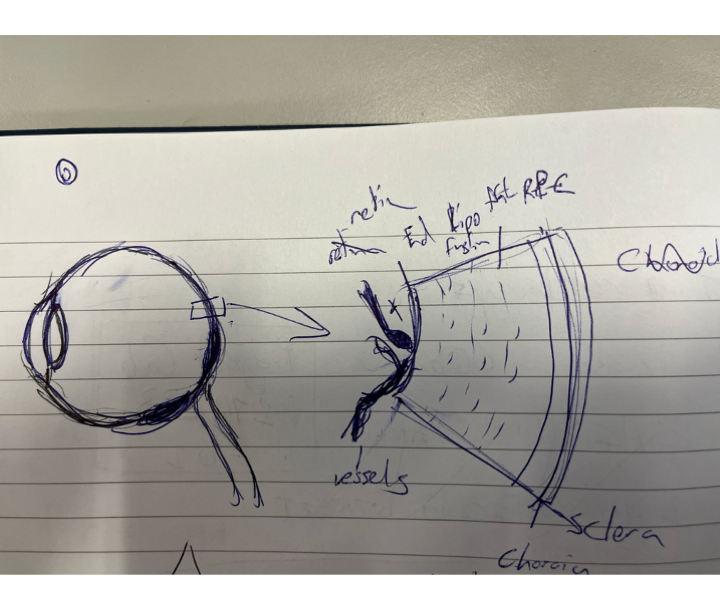
\includegraphics[width = 0.8\textwidth]{Figures/EyeStructure.png}
    \caption{The retina comprises of multiple sections which can be affected by disease. Fluorescent biomarkers are distributed amongst multiple layers and the emitted fluorescence experiences scattering, re-emission between these layers and further interaction with blood vessels before it can be detected.
    \textcolor{blue}{My deepest apologies for this poorly drawn figure and my handwriting/Sanskrit. But think this conveys roughly what it should show i.e the multiple layers of the retina and where the fluorophores are distributed}}
    \label{fig:eyestructure}
\end{figure}



\begin{figure}
    \centering
    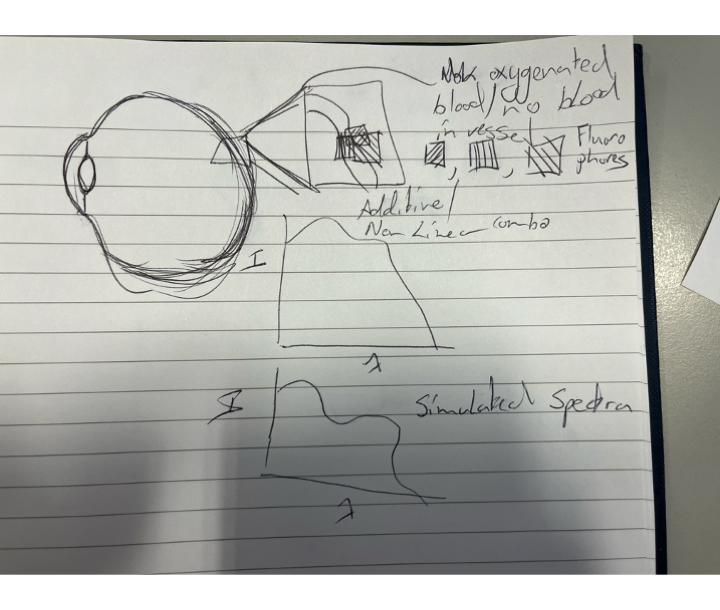
\includegraphics[width = 0.8\textwidth]{Figures/ModelValidation.png}
    \caption{The influence of blood vessels on the measure spectra of retina images is examined by simulating a mixture of known retinal fluorophores distributed between multiple layers of the retina with and without a blood vessel, containing oxygenated blood, situated axially above. The measured spectra produced from the Monte Carlo simulations, and from a rudimentary linear combination are shown.[insert results here] \textcolor{blue}{This is also poorly drawn but I think the way to demonstrate the spectral effects of blood vessels and oxygenated blood on the fluorescence from e.g FAD is to simply run a simulation with and with out blood vessels}}
    \label{fig:modelvalidation}
\end{figure}


\subsection{Phasor S-FLIM}

\begin{outline}
    \1 Introduce phasor analysis and the phasor plot
        \2 Phasor analysis is a method of extracting fluoresence lifeimes from FLIM dats using Fourier Transforms
        \2 Un-like standard fitting based approached it is not susceptible to user bias / reliant on the user to select the correct number of exponential decays to fit to
        \2 Phasor analysis is computationally cheaper by only requiring a single FFT per pixel per $\lambda$ channel compared to iterative re-convolution fitting on a per pixel per $\lambda$ basis
        \2 See Equation\ref{eq:phasortransform}
        \2 See Equation \ref{eq:reconvfitting}
    \1 S-FLIM unmixing algorithm
        \2 FLIM data for each $\lambda$ is either captured sequentially over multiple exposures, in the case of SPAD arrays where a FLimage is obtained for each spectral channel. Alternatively a line SPAD array can be used with a scanning based system with the fluorescence being spectrally separated using a diffraction grating and the image is built up by raster scanning across the scene.
        \2 The temporal response of the system, or the Instrument Response Function, is accounted for for in phasor space. Deconvolution becomes a simple scaling, and rotation of the phasor
        \2 The Endmembers are identified on the phasor plot using principle components
        \2 The endmember spectra are then recovered and the relative concentration of the fluorophore can be determined.
\end{outline}

\begin{align}
    g(x,y,\lambda) &= \frac{\int_{-\infty}^{\infty}I(t)\cos{(\omega t)dt}}{\int_{-\infty}^{\infty}I(t)} \equiv \frac{\mathcal{R}\big(\mathcal{F}\{I(t)\}\rvert_{n=1}\big)}{\mathcal{F}\{I(t)\}\rvert_{n=0}\big)}\\
    s(x,y,\lambda) &= \frac{\int_{-\infty}^{\infty}I(t)\sin{(\omega t)dt}}{\int_{-\infty}^{\infty}I(t)} \equiv \frac{\mathcal{I}\big(\mathcal{F}\{I(t)\}\rvert_{n=1}\big)}{\mathcal{F}\{I(t)\}\rvert_{n=0}\big)}\\
    \label{eq:phasortransform}
\end{align}

\begin{equation}
    \{c_{i}, \tau_{i}\} = min\bigg\{\text{data} - \text{IRF}\otimes\sum_{n > 0}c_{i}(\nicefrac{-t}{\tau_{i}}) \bigg\}
    \label{eq:reconvfitting}
\end{equation}

\begin{figure}[h!]
    \centering
    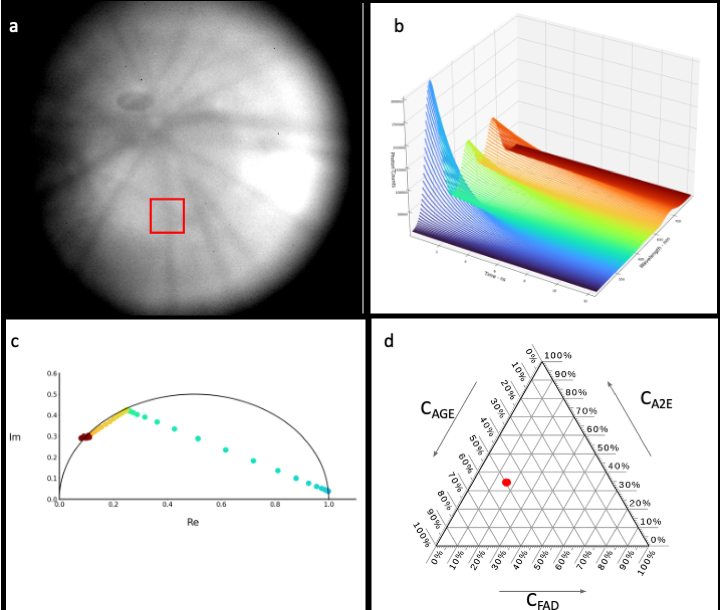
\includegraphics[width = 0.8\textwidth]{Figures/MockSFLIM2.png}
    \caption{a) Example fluorescence intensity image generated using the multilayered model comprising of multiple fluorophores/chromophores interacting non-additively  b) In the highlighted region the spectrally, and temporally resolved fluorescence signals are generated using our multilayered model where various endogenous fluorophores interact additively and non additively. This is collated into a single S-FLIM pixel. c) The S-FLIM dataset is then represented in phasor space using the first harmonic of the Fourier Transform d) The unmixing algorithm then recovers the relative concentrations of the constituent fluorophores.\\
    \textcolor{blue}{This is a really rough idea for one of the captions where it shows the outputs from each step of the S-FLIM unmixing process. I think a ternary plot might a good way to show the relative concentrations of each fluorophore but does absorption/scattering due to vessels imply $c_{AGE} + c_{A2E} + c_{FAD} = 100\%?$}}
    \label{fig:sflim}
\end{figure}



\subsection{Feasibility of Detecting Fluorophores}
\begin{outline}
    \1 The SNR of the FLIM measurements will limit the accuracy and precision of the recovery of relative fluorophore abundance, and thus the estimated concentration \textcolor{blue}{I feel there is a better term to distinguish between the relative concentration of a fluorophore in the fluorescence signal, \% , and the actual physical quantity of the chemical, ppm / mol per cm3 etc?}
    \1 The noise inherent in the FLIM signal can initially be simulated using a simple Poissionian / shot noise model but can also be extended to account for dark counts, read noise, after-pulsing using \cite{dutton2016single} Eq \ref{eq:fluorescencemodel} 
    \1 With this noise model and determining the imaging efficiency of the retina the integration time and/or detector sensitivity required for a given precision of fluorophore quantification can be estimated.
    \1 These results will be used to define whether we are hindered by the sensitivity of the detectors or some limit of biology. 

    

\end{outline}

\begin{equation}
I(t) = \text{IRF}\otimes I_{0}\sum_{i > 0}^{N}c_{i}\exp{\bigg (\nicefrac{-t}{\tau_{i}}} \bigg)
    \label{eq:fluorescencemodel}
\end{equation}


\section{Results/ Discussion}
\textcolor{blue}{I've only given vague bullet points for this section since we don't know the outcomes yet.}
\begin{outline}
        \1 These biological limits would be framed in the terms of safe exposure limits, or some arbitrary time limit to record an image
            \2 Is the expected concentration of the target fluorophore too small compared to he uncertainties in the unmixing algorithm. i.e. $\Delta c_{i} > c_{i}$
            \2 Is the required integration time, dictated by safe exposure limits, on the order of hours/days such that it wouldn't be feasible in a commercial device used in regular practise. 
            \2 (Assuming the unmixing works) what are the uncertainties at different photon fluxes, what variation in fluorophore concentrations can we reliably / repeatably measure. See mock Fig. \ref{fig:sflimperformance}
            \2 A graph of the expected / simulated number of photons per second that are incident on the detector as a function of time should be simulated and plotted in this section. This would help put into context the precision vs. photon number value we are looking at
        \1 The concentrations we can reliable extract, and the variability can also be explained in terms of the expected variation in FAD concentrations we might see with the progression of retina disease, oxygenation etc.
        \1 The role of the detector should in this variability should also be explained - i.e if we instead had a SPAD with 90\% fill factor how would this improve the unmixing process.
\end{outline}

\begin{figure}
    \centering
    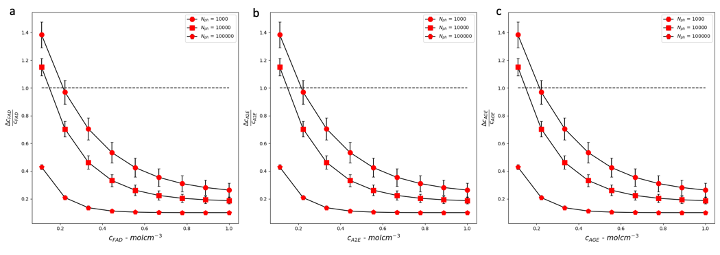
\includegraphics[width = \textwidth]{Figures/SFLIMPerformance.png}
    \caption{The accuracy and precision of the unmixing algorithm are evaluated for FAD (a), AGE (b), and A2E/lipofuscin (c) using the Monte Carlo ray tracing simulations. The performance is characterised in terms the uncertainty $\Delta c_{i}$ as a fraction of the recovered concentration, $c_{i}$ and over multiple photon counts per $\lambda$ channel, $N_{ph}$. \textcolor{blue}{This captions needs a lot of work but esseintially what I think it should show and explain is the fractional uncertainty (or some other suitable metric such as RMS error) in the recovered concentrations as a function of the concentration. The y = 1 line denotes where our uncertainty in the recovered value is the same as the value}}
    \label{fig:sflimperformance}
\end{figure}
\bibliography{bibliography.bib}





\end{document}
